% --------------------------------------------------------------
% This is all preamble stuff that you don't have to worry about.
% Head down to where it says "Start here"
% --------------------------------------------------------------
 
\documentclass[12pt]{article}
 
\usepackage[margin=1in]{geometry} 
\usepackage{amsmath,amsthm,amssymb}
 
\newcommand{\N}{\mathbb{N}}
\newcommand{\Z}{\mathbb{Z}}
 
\newenvironment{theorem}[2][Theorem]{\begin{trivlist}
\item[\hskip \labelsep {\bfseries #1}\hskip \labelsep {\bfseries #2.}]}{\end{trivlist}}

\newenvironment{lemma}[2][Lemma]{\begin{trivlist}
\item[\hskip \labelsep {\bfseries #1}\hskip \labelsep {\bfseries #2.}]}{\end{trivlist}}

\newenvironment{exercise}[2][Exercise]{\begin{trivlist}
\item[\hskip \labelsep {\bfseries #1}\hskip \labelsep {\bfseries #2.}]}{\end{trivlist}}

\newenvironment{problem}[2][Part]{\begin{trivlist}
\item[\hskip \labelsep {\bfseries #1}\hskip \labelsep {\bfseries #2}]}{\end{trivlist}}

\newenvironment{intro}[2][Introduction]{\begin{trivlist}
\item[\hskip \labelsep {\bfseries #1}\hskip \labelsep {\bfseries #2}]}{\end{trivlist}}

\newenvironment{question}[2][Question]{\begin{trivlist}
\item[\hskip \labelsep {\bfseries #1}\hskip \labelsep {\bfseries #2.}]}{\end{trivlist}}

\newenvironment{corollary}[2][Corollary]{\begin{trivlist}
\item[\hskip \labelsep {\bfseries #1}\hskip \labelsep {\bfseries #2.}]}{\end{trivlist}}

\usepackage{graphicx}
\graphicspath{{./}}

\newcommand{\bestBeta}{0.4}

\begin{document}
 
% --------------------------------------------------------------
%                         Start here
% --------------------------------------------------------------
 
\title{Project 2: Image Inpainting with MRF}%replace X with the appropriate number
\author{Yunzhong He\\ %replace with your name
204010749} %if necessary, replace with your course title
 
\maketitle

\begin{problem}{I Introduction}
\item{}
The project is to restore a distorted image given the location of its masked region. For the masked region, we modeled its distribution as a MRF model given by 
\begin{align*}
	p(X_\Lambda|X_{\partial\Lambda}) = \frac{1}{Z}exp(-\beta\sum_{(x,y)\in\Lambda} (E(\nabla_x) + E(\nabla_y)))
\end{align*}
Where $E$ is an energy function, we tried $L_1$ and $L_2$ norms for $E$.
\begin{align*}
	&E_1(\nabla_x(x, y)) = |\nabla_xX(x,y)|\\
	&E_2(\nabla_x(x, y)) = (\nabla_xX(x,y))^2
\end{align*}
And for this project, we only look at the red channel of the image. After inpainting the masked region, we used the squared error per pixel against the original image $Err = \frac{1}{\Lambda} \sum (X(x,y) - O(x,y))^2$ to measure the accuracy.
\end{problem}

\begin{problem}{II Gibbs Sampler}
\item{}
For a given joint distribution of the masked region as in Part I, we want to randomly sample its values $X_\Lambda$ to inplant this region. But due to the dimionsionality of the distribution, we used Gibbs sampler to sample the image pixel by pixel, and performed up to 20 sweeps.\\

\item{II.1 L-1 Norm\\}
Before sampling, we tuned $\beta$ with several sweeps, and picked $\beta$ to be \bestBeta \ for all further samplings. And below are the reconstucted red channel after 20 sweeps, and the per pixel error against each sweep.
\begin{center}
	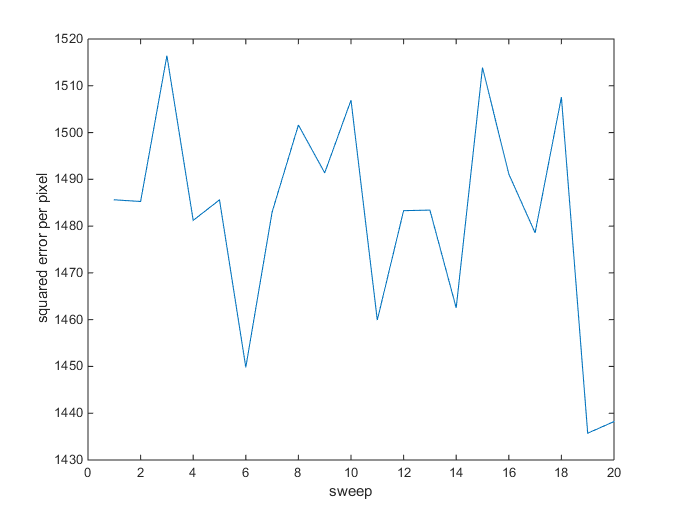
\includegraphics[width=14cm]{results/error_gibbs_04.png}{\\figure 1 squared error per pixel against sweeps}
	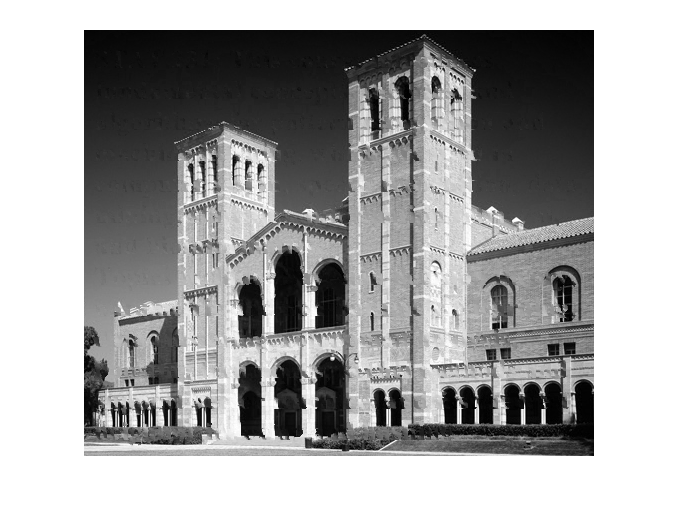
\includegraphics[width=14cm]{results/recover_gibbs_04.png}{\\figure 2 recovered image after 20 sweeps}
\end{center}

\item{II.2 L-2 Norm\\}
We also performed the same procedure using L-2 norm as our energy function, and obtained the following results.
\begin{center}
	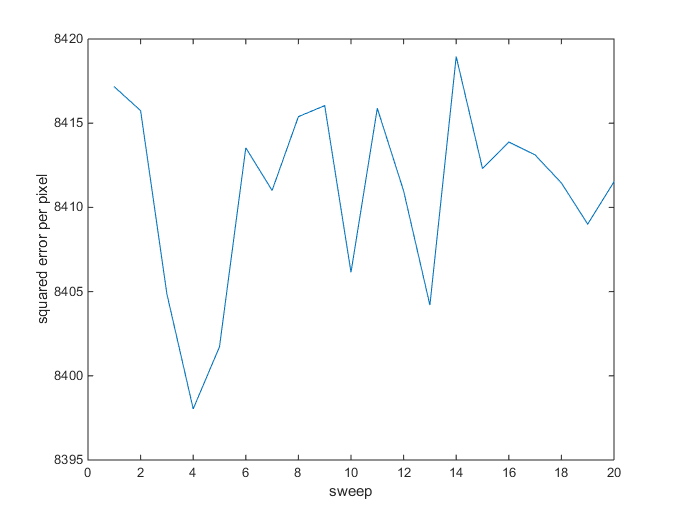
\includegraphics[width=14cm]{results/error_gibbs_l2.png}{\\figure 3 squared error per pixel against sweeps}
	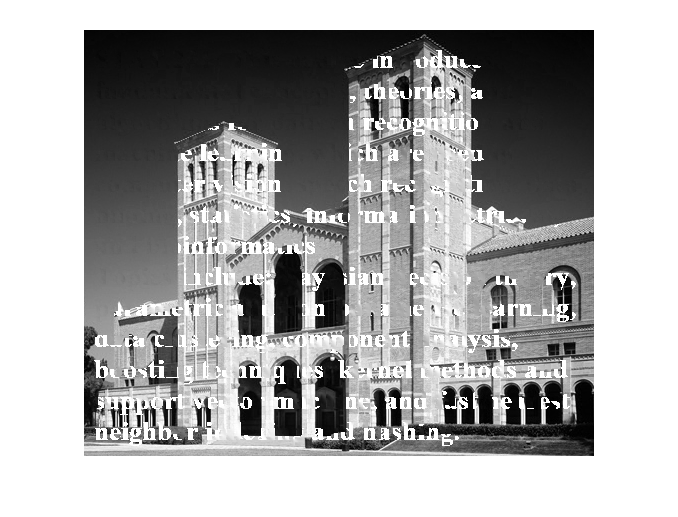
\includegraphics[width=14cm]{results/gibbs_recover_l2.png}{\\figure 4 recovered image after 20 sweeps}
\end{center}

\item{II.3 Analysis}
Comparing the results from II.1 and II.2 we can see that L-1 norm yields lower error and better recovery result. This may due to the face that L-2 norm is smoother near optima, which makes results that are relativly good more likely to be sampled, and therefore reduce the probability of results near optima to be sampled.
\end{problem}

\begin{problem}{III PDE}
\item{III.1 Gradient Descent\\}
An alternative way to find $X(x,y)$ is through gradient descent, as earier we proved that with L-2 norm, the gradient of an image change is given by the heat-difussion equation.
\begin{align*}
	\frac{dX(x,y,t)}{dt} = \Delta X(x,y)
\end{align*}
We tuned also tuned the parameter $\beta$ and found $\beta = 0.2$ works very well in terms of gradient descent. Below are the results.
\begin{center}
	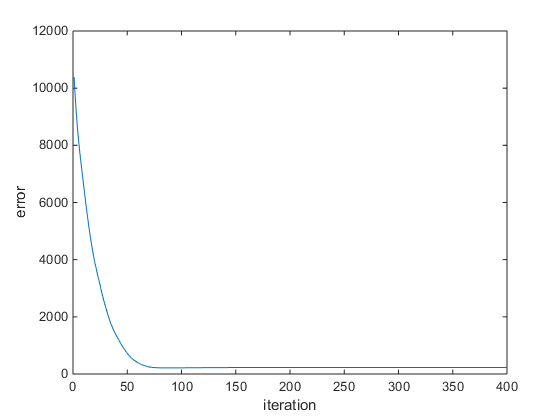
\includegraphics[width=14cm]{results/error_heat_diffusion.png}{\\figure 5 squared error per pixel against iteration}
	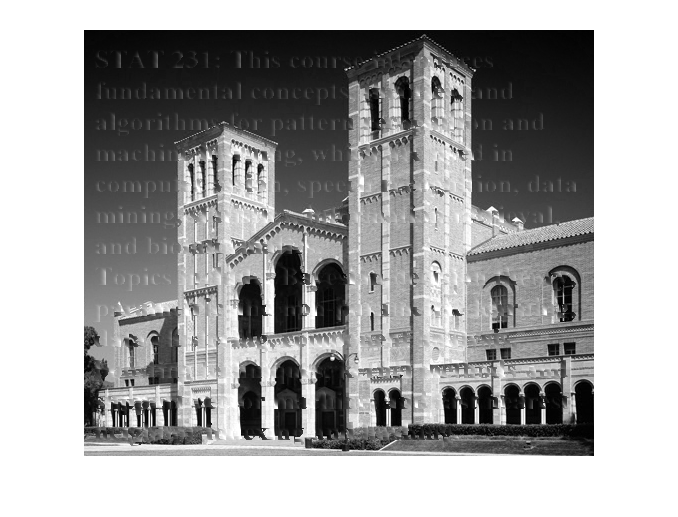
\includegraphics[width=14cm]{results/recover_heat_diffusion.png}{\\figure 6 recovered image through PDE}
\end{center}

\item{III.2 Analysis\\}
Comparing the results from II.2 we can see the PDE method clearly generates lower error and better recovered image. This is because with $beta$ good enrough, gradient descent always reduces the error at next iteration, unlike the Gibbs sampling method where the error may increase at the next sweep. So the fact that L-2 norm having smooth boundary near optima can be overcome by having more iterations, and thus better results can be achieved.
\end{problem}

% --------------------------------------------------------------
%     You don't have to mess with anything below this line.
% --------------------------------------------------------------
 
\end{document}
